\section{Use case diagram}
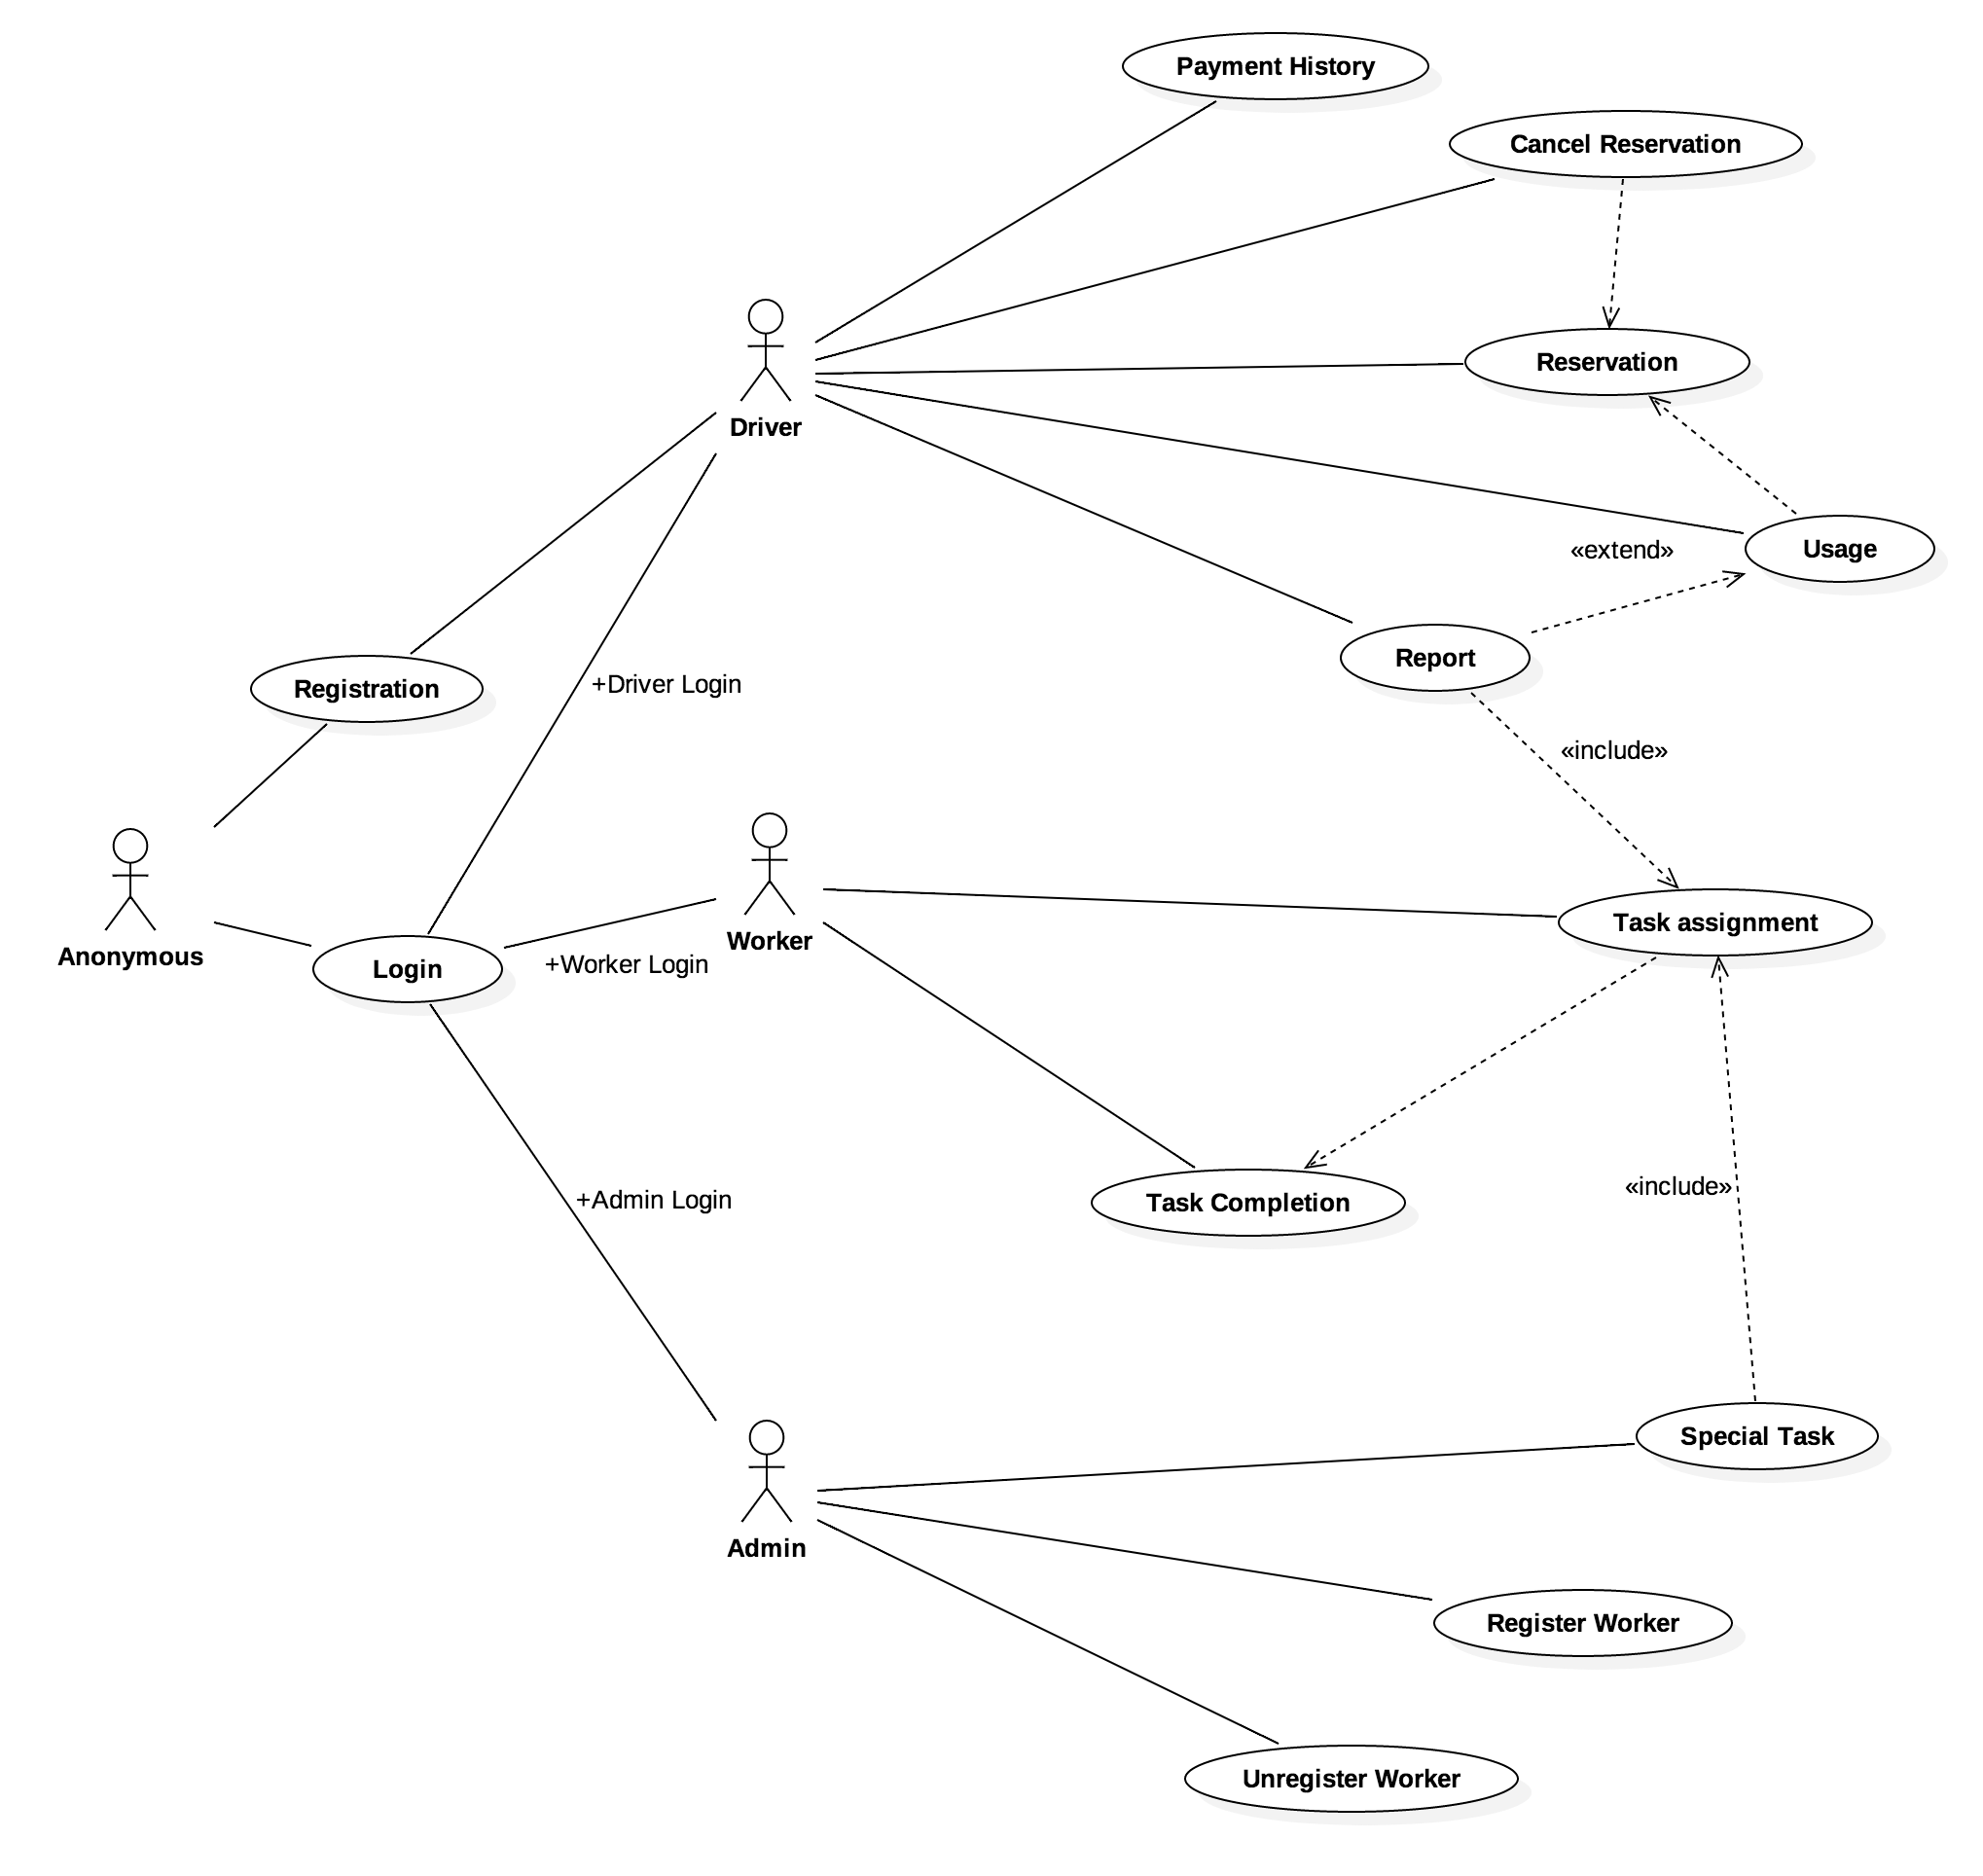
\includegraphics[width=13cm,height=13cm,keepaspectratio]{usecase}
\section{Driver use cases}
Here we list relevant use cases for the Driver:\\
\begin{center}
\noindent\rule{8cm}{1.0pt}
\end{center}

\textbf{\large Driver registration}
\bigbreak
\textbf{Name:} Driver registration \\
\textbf{Actors:} Driver \\
\textbf{Entry conditions:} 
\begin{itemize}
\item The Driver has already downloaded the application or he/she is on the web portal.
\end{itemize}
\textbf{Flow of events:} 
\begin{itemize}
\item The Driver provides an email and a password;
\item The Driver provides information about himself/herself (full name, date of birth, address, sex);
\item The Driver clicks the sign up button;
\item The System verifies if the email is valid and not already in use;
\item The System verifies if the password matches the rules (lenght, special characters);
\item The System asks for driving license and payment information;
\item The Driver uploads pictures of his license and credit card;
\item The System shows a "success" message and sends a confirmation email.
\end{itemize}
\textbf{Exit conditions:} the Driver is registered and logged into the system.\\
\textbf{Exceptions:} 
\begin{itemize}
\item If submitted data is not valid the System asks for them again.
\end{itemize}

\begin{center}
\noindent\rule{8cm}{1.0pt}
\end{center}


\textbf{\large Driver login}
\bigbreak
\textbf{Name:} Driver login \\
\textbf{Actors:} Driver \\
\textbf{Entry conditions:} 
\begin{itemize}
\item The Driver has already downloaded the application or he/she is on the web portal.
\end{itemize}
\textbf{Flow of events:} 
\begin{itemize}
\item The Driver provides username and password;
\item The Driver clicks the login button;
\item The System verifies the credentials.
\end{itemize}
\textbf{Exit conditions:} the Driver is logged into the system.\\
\textbf{Exceptions:} 
\begin{itemize}
\item If credentials are wrong the system asks for them again.
\end{itemize}


\begin{center}
\noindent\rule{8cm}{1.0pt}
\end{center}


\textbf{\large Car reservation}
\bigbreak
\textbf{Name:} Car reservation \\
\textbf{Actors:} Driver \\
\textbf{Entry conditions:} 
\begin{itemize}
\item The Driver is logged in;
\item The Driver must not be a Blocked Driver.
\end{itemize}
\textbf{Flow of events:} 
\begin{itemize}
\item The System automatically fetches the Driver's position and presents a list of available nearby cars;
\item The Driver selects one of the available cars;
\item The System pre-authorizes the fixed amount from the credit card and marks the car as reserved;
\item The System shows a "success" message and sends an email with reservation information (car location, car plate, cancel reservation link)
\end{itemize}
\textbf{Exit conditions:} 
\begin{itemize}
\item The Driver has a reservation and cannot reserve other cars 
\item The car is not available for other Drivers.\\
\end{itemize}
\textbf{Exceptions:} 
\begin{itemize}
\item If the Driver does not have enough money the reservation in not successful.
\end{itemize}


\begin{center}
\noindent\rule{8cm}{1.0pt}
\end{center}


\textbf{\large Driver uses the service}
\bigbreak
\textbf{Name:} Driver uses the service\\
\textbf{Actors:} Driver \\
\textbf{Entry conditions:} 
\begin{itemize}
\item The Driver has already reserved a car.
\end{itemize}
\textbf{Flow of events:} 
\begin{itemize}
\item The System waits till the user is nearby the car then enables the open button on the application;
\item The Driver opens the car by pressing the button;
\item The Driver gets inside the car, turns it on and begins to drive;
\item The System logs the route and the duration of the drive;
\item The System presents to the Driver his current due amount and all the nearby recharging stations;
\item The Driver stops the car, gets outside the car and closes the door;
\item 30 seconds later the car automatically locks itself and the ride is terminated by the System;
\item The System calculates the correct amount to be paid (depending on discount policies) and charges the Driver's credit card accordingly.
\end{itemize}
\textbf{Exit conditions:} the Driver got to the final destination and the car is marked again as "available".\\
\textbf{Exceptions:}  
\begin{itemize}
\item If the Driver does not start his ride within one hour, the reservation expires and his credit card is charged 1 Euro and the car status is reset to "available". 
\end{itemize}

\begin{center}
\noindent\rule{8cm}{1.0pt}
\end{center}


\textbf{\large Cancel reservation}
\bigbreak
\textbf{Name:} Cancel reservation\\
\textbf{Actors:} Driver \\
\textbf{Entry conditions:} 
\begin{itemize}
\item The Driver has already reserved a car;
\item The reservation happened within one hour.
\end{itemize}
\textbf{Flow of events:} 
\begin{itemize}
\item The user clicks either on the "cancel reservation" button on the application or on the "cancel reservation" link provided in the reservation email;
\item The System cancels the reservation without charging the user.
\end{itemize}
\textbf{Exit conditions:} 
\begin{itemize}
\item The car is marked as "available" again;
\item The Driver can reserve cars again.
\end{itemize}
\textbf{Exceptions:} there are no exceptions for this use case.\\


\begin{center}
\noindent\rule{8cm}{1.0pt}
\end{center}


\textbf{\large Report a problem}
\bigbreak
\textbf{Name:} Report a problem\\
\textbf{Actors:} Driver \\
\textbf{Entry conditions:} 
\begin{itemize}
\item The Driver started his ride;
\item The car has a problem.
\end{itemize}
\textbf{Flow of events:} 
\begin{itemize}
\item The Driver clicks on the "report" button and specifies the type of problem; 
\item The ride terminates and the Driver pays accordingly;
\item The Driver gets outside the car.
\end{itemize}
\textbf{Exit conditions:} 
\begin{itemize}
\item A Task is generated and is assigned to the most suitable available Worker;
\item The Driver can reserve cars again.
\end{itemize}
\textbf{Exceptions:} there are no exceptions for this use case.\\


\begin{center}
\noindent\rule{8cm}{1.0pt}
\end{center}



\textbf{\large View payment history}
\bigbreak
\textbf{Name:} View payment history\\
\textbf{Actors:} Driver \\
\textbf{Entry conditions:} 
\begin{itemize}
\item The Driver is logged into the System.
\end{itemize}
\textbf{Flow of events:} 
\begin{itemize}
\item The Driver clicks on the Personal History button inside the web portal
\item The System presents a detailed log of all the previous reservation and payments.
\end{itemize}
\textbf{Exit conditions:} 
\begin{itemize}
\item The Driver is informed on his/her history.
\end{itemize}
\textbf{Exceptions:} there are no exceptions for this use case.\\


\begin{center}
\noindent\rule{8cm}{1.0pt}
\end{center}



\section{Worker use cases}
Here we list relevant use cases for the Worker:\\
\begin{center}
\noindent\rule{8cm}{1.0pt}
\end{center}


\textbf{\large Worker login}
\bigbreak
\textbf{Name:} Worker login \\
\textbf{Actors:} Worker \\
\textbf{Entry conditions:} 
\begin{itemize}
\item The Worker has already downloaded the application;
\item The Worker has been registered by an Admin.
\end{itemize}
\textbf{Flow of events:} 
\begin{itemize}
\item The Worker places the NFC badge on his phone;
\end{itemize}
\textbf{Exit conditions:} 
\begin{itemize}
\item The Worker is logged into the system and his workday begins.
\end{itemize}
\textbf{Exceptions:} there are no exceptions for this use case.\\


\begin{center}
\noindent\rule{8cm}{1.0pt}
\end{center}


\textbf{\large Task assignment}
\bigbreak
\textbf{Name:} Task assignment\\
\textbf{Actors:} Worker \\
\textbf{Entry conditions:} 
\begin{itemize}
\item The Worker is logged into the System;
\item The Worker is available;
\item The System generated a Task which has not been assigned yet.
\end{itemize}
\textbf{Flow of events:} 
\begin{itemize}
\item The System chooses the most suitable available Worker depending on its policies (distance, workload, van batteries);
\item The System notifies with a push notification the selected Worker and sends him all the needed information (location, type of task, car info).
\end{itemize}
\textbf{Exit conditions:} 
\begin{itemize}
\item The Task is assigned to the worker;
\item The Worker is marked as busy.
\end{itemize}
\textbf{Exceptions:} there are no exceptions for this use case.\\



\begin{center}
\noindent\rule{8cm}{1.0pt}
\end{center}


\textbf{\large Task completion}
\bigbreak
\textbf{Name:} Task completion\\
\textbf{Actors:} Worker \\
\textbf{Entry conditions:} 
\begin{itemize}
\item The Worker has been assigned a Task;
\item The Worker completed the task;
\end{itemize}
\textbf{Flow of events:} 
\begin{itemize}
\item The Worker informs the System that the work has been completed using the application;
\end{itemize}
\textbf{Exit conditions:} 
\begin{itemize}
\item The Worker is marked as available again;
\end{itemize}
\textbf{Exceptions:} 
\begin{itemize}
\item If the Worker did not manage to complete the Task he closes the Task providing a description. The System Admin will manage the situation manually (e.g. calling a tow truck).
\end{itemize}


\begin{center}
\noindent\rule{8cm}{1.0pt}
\end{center}


\section{Admin use cases}
Here we list relevant use cases for the Admin:\\
\begin{center}
\noindent\rule{8cm}{1.0pt}
\end{center}


\textbf{\large Admin login}
\bigbreak
\textbf{Name:} Admin login \\
\textbf{Actors:} Admin \\
\textbf{Entry conditions:} there are no entry conditions for this use case.\\
\textbf{Flow of events:} 
\begin{itemize}
\item The Admin provides his credentials to the System  
\end{itemize}
\textbf{Exit conditions:} 
\begin{itemize}
\item The Admin is logged into the System.
\end{itemize}
\textbf{Exceptions:} there are no exceptions for this use case.\\


\begin{center}
\noindent\rule{8cm}{1.0pt}
\end{center}


\textbf{\large Register employee}
\bigbreak
\textbf{Name:} Register employee \\
\textbf{Actors:} Admin \\
\textbf{Entry conditions:} 
\begin{itemize}
\item The Admin is logged into the System.
\end{itemize}
\textbf{Flow of events:} 
\begin{itemize}
\item The Admin provides the new employee's information to the System (full name, ID);
 \item The System prints the new Worker's badge and writes a unique NFC signature on it.
\end{itemize}
\textbf{Exit conditions:} 
\begin{itemize}
\item The new Worker is registered.
\end{itemize}
\textbf{Exceptions:} there are no exceptions for this use case.\\


\begin{center}
\noindent\rule{8cm}{1.0pt}
\end{center}


\textbf{\large Unregister employee}
\bigbreak
\textbf{Name:} unregister employee \\
\textbf{Actors:} Admin \\
\textbf{Entry conditions:} 
\begin{itemize}
\item The Worker has been fired or reassigned.
\end{itemize}
\textbf{Flow of events:} 
\begin{itemize}
\item The Admin selects the employee to be unregistered.
\end{itemize}
\textbf{Exit conditions:} 
\begin{itemize}
\item The Worker is no more registered and his credentials are invalidated.
\end{itemize}
\textbf{Exceptions:} there are no exceptions for this use case.\\


\begin{center}
\noindent\rule{8cm}{1.0pt}
\end{center}


\textbf{\large Get analytics}
\bigbreak
\textbf{Name:} get analytics \\
\textbf{Actors:} Admin \\
\textbf{Entry conditions:} 
\begin{itemize}
\item The Admin is logged in.
\end{itemize}
\textbf{Flow of events:} 
\begin{itemize}
\item The Admin selects the car or the worker to get analytics of;
\end{itemize}
\textbf{Exit conditions:} 
\begin{itemize}
\item The System shows detailed analytics
\end{itemize}
\textbf{Exceptions:} there are no exceptions for this use case.\\


\begin{center}
\noindent\rule{8cm}{1.0pt}
\end{center}


\textbf{\large Request special Task}
\bigbreak
\textbf{Name:} request special Task \\
\textbf{Actors:} Admin \\
\textbf{Entry conditions:} 
\begin{itemize}
\item The Admin is logged in.
\end{itemize}
\textbf{Flow of events:} 
\begin{itemize}
\item The Admin writes a description of the special Task, including the car ID.
\end{itemize}
\textbf{Exit conditions:} 
\begin{itemize}
\item A Worker is notified.
\end{itemize}
\textbf{Exceptions:} there are no exceptions for this use case.\\


\begin{center}
\noindent\rule{8cm}{1.0pt}
\end{center}
